\tocslide
\subsection{Aim}
\begin{frame}
  \rfn
  \frametitle{Project task}
  Simple solenoid lens design:
  \begin{itemize}
    \item Monochromatic \textit{e} beam, fixed beam radius $R$
    \item Target FWHM, peak $B_z$, $f$
    \item Optimize geometry, current for minimal aberrations
  \end{itemize}
  \begin{figure}
    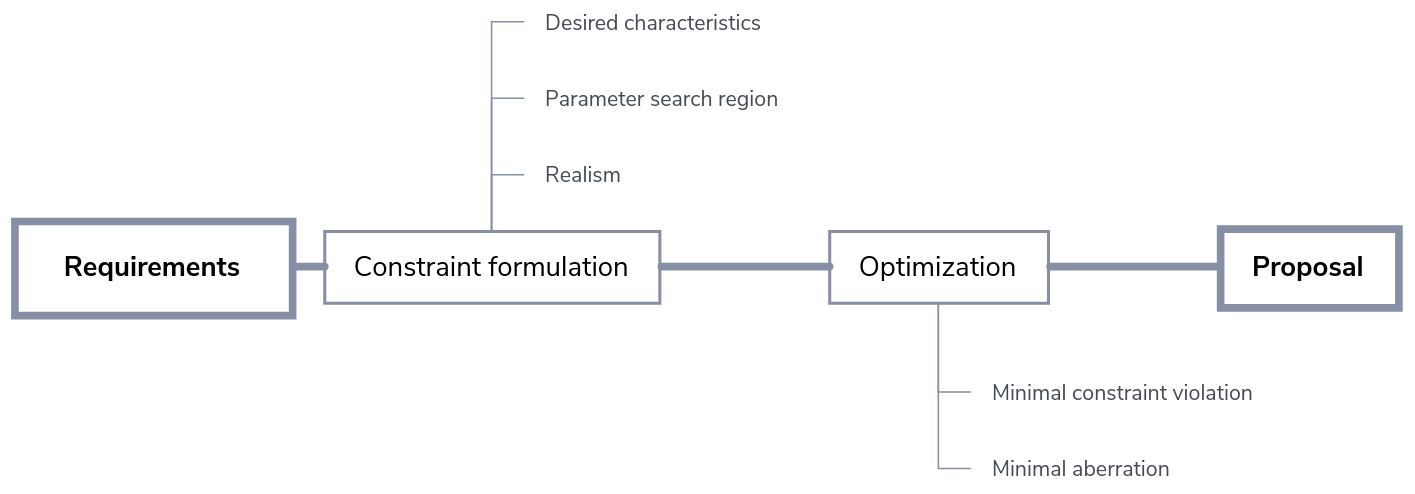
\includegraphics[width=\textwidth]{blok_cxema}
    \caption{Generalized design process}
  \end{figure}
\end{frame}

\subsection{Model}
\begin{frame}
  \rfn
  \frametitle{Solenoid model}
  \begin{itemize}
    \item Rectangular cross-section solenoid\footcite{Disser}
  \end{itemize}
  \begin{columns}
    \begin{column}{0.6\textwidth}
      Two-loop field approximation:
      \begin{small}
      \begin{center}
        \[
        B_{z}\left(z\right)\approx\frac{\mu_{0}NI}{4}\left(\frac{Rc^{2}}{\left(z^{2}+Rc^{2}\right)^{3/2}}+\frac{Rc^{*2}}{\left(z^{2}+Rc^{*2}\right)^{3/2}}\right);
        \]
        \[
        Rc = R_{sq}+c,\ \text{where}\
        c^{2} = \frac{b^{2}-a^{2}}{12},
        \]
        \[
        R_{sq} = R_{m}\left(1+\frac{a^{2}}{24R_{m}^{2}}\right).
        \]
      \end{center}
      \end{small}
    \end{column}
    \begin{column}{0.4\textwidth}
      \begin{figure}
        \centering
        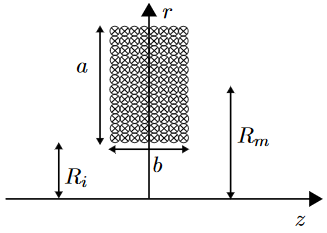
\includegraphics[width=\textwidth]{Multilay_solenoid2}
        \caption{Solenoid geometry:\\
        $R_m$ - mean radius\\
        $a$ - transverse width\\
        $b$ - axial length
        }
      \end{figure}
    \end{column}
  \end{columns}
  \vspace{0.25cm}
  Parameters: geometry, scaling factor $N\cdot I$ [Ampere-Turns]
\end{frame}

\begin{frame}
  \rfn
  \frametitle{Field integrals}
  For an axial beam, only the on-axis $B_z$ is of significance\footcite{Disser}. The field's optical properties are described in terms of:
  \begin{columns}
    \begin{column}{0.5\textwidth}
      \begin{center}
      \begin{small}
        \[F_1 = \int B_z dz\]
        \[F_2 = \int B_z^2 dz\]
      \end{small}
      \end{center}
    \end{column}
    \begin{column}{0.5\textwidth}
      \begin{center}
      \begin{small}
      \[F_3 = \int - \frac{B_z''\cdot B_z}{2} dz \]
      \[F_4 = \int B_z^4 dz\]
      \end{small}
      \end{center}
    \end{column}
  \end{columns}
  \vspace{1cm}
  whereas the integration domain is ($-\infty,\infty$).
\end{frame}

\begin{frame}
  \rfn
  \frametitle{Solenoid characteristics}
    \begin{itemize}
      \item Peak $B_z = B_z(0)$; effective field length $\rightleftarrows$ FWHM
      \item Focal length:
        \begin{small}
          \[
          f = \left(\frac{2p_z}{e}\right)^2\frac{1}{F_2}
          \]
        \end{small}
      \item Spherical aberration coefficient:
        \begin{small}
          \[
          c_s = \frac{e^{2}R^{4}}{4p_{z,0}^{2}}F_{3}+\frac{e^{4}R^{4}}{12p_{z,0}^{4}}F_{4}
          \]
        \end{small}
      \item Resulting focal spot size:
        \begin{small}
        \[
        r_{s}=C_{s}\cdotp\left(\frac{r_{in}}{f-\frac{C_{s}r_{in}^{2}}{f^{2}}}\right)^{3}
        \]
        \end{small}
    \end{itemize}
    \vspace{0.5cm}
    Considerations:
    \begin{itemize}
      \item  - size, material usage
      \item Scaling factor, geometry - power consumption, material usage
      \item $f$, FWHM, $c_s$, $r_s$: interaction with other components, lens quality
    \end{itemize}
\end{frame}


\subsection{Optimization}
\begin{frame}
  \frametitle{Optimization}
  We used:
  \begin{itemize}
    \item Constrained Trust Region algorithm\footcite{scipyctr} - minimize $c_s$ and constraint violation with dynamic \textquotedblleft trust region\textquotedblright definition
    \item Interior Point algorithm: \footcite{byrd2000trust} - a more rigorous, less flexible implementation of the \textquotedblleft trust region\textquotedblright concept
  \end{itemize}
  \vspace{0.5cm}
  \begin{figure}
    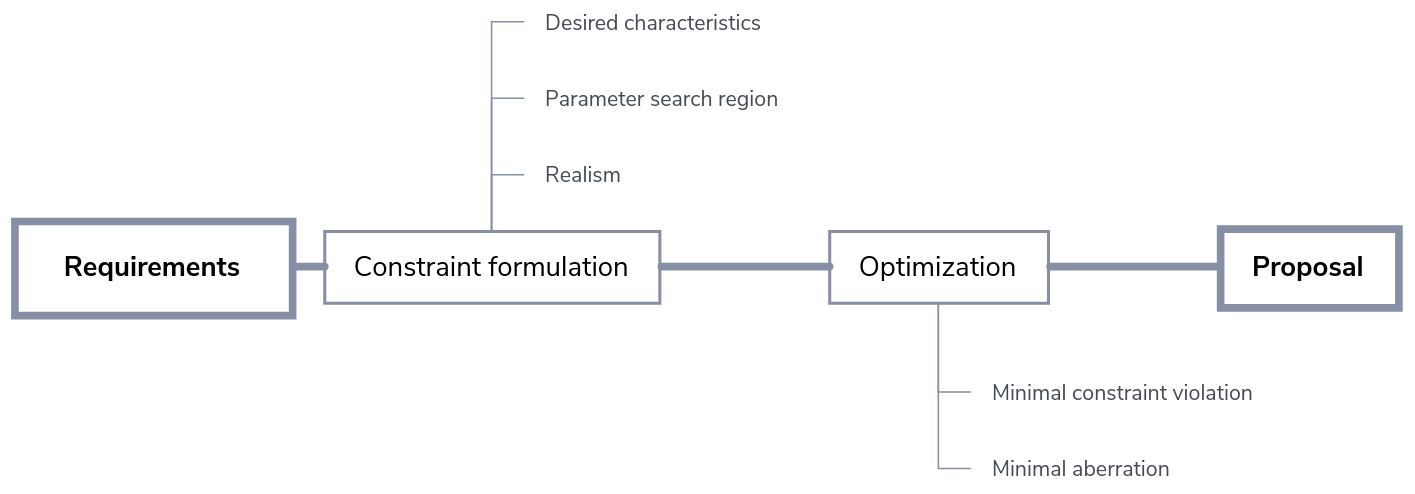
\includegraphics[width=0.9\textwidth]{blok_cxema}
  \end{figure}
\end{frame}
